\documentclass[tikz,border=10pt]{standalone}
\usetikzlibrary{shapes.geometric, arrows.meta, positioning, fit, backgrounds, calc}

% --- CHUẨN HOÁ PHÔNG CHỮ IEEE (Helvetica / Arial Sans-Serif) ---
\usepackage{helvet}
\renewcommand{\familydefault}{\sfdefault}

\begin{document}
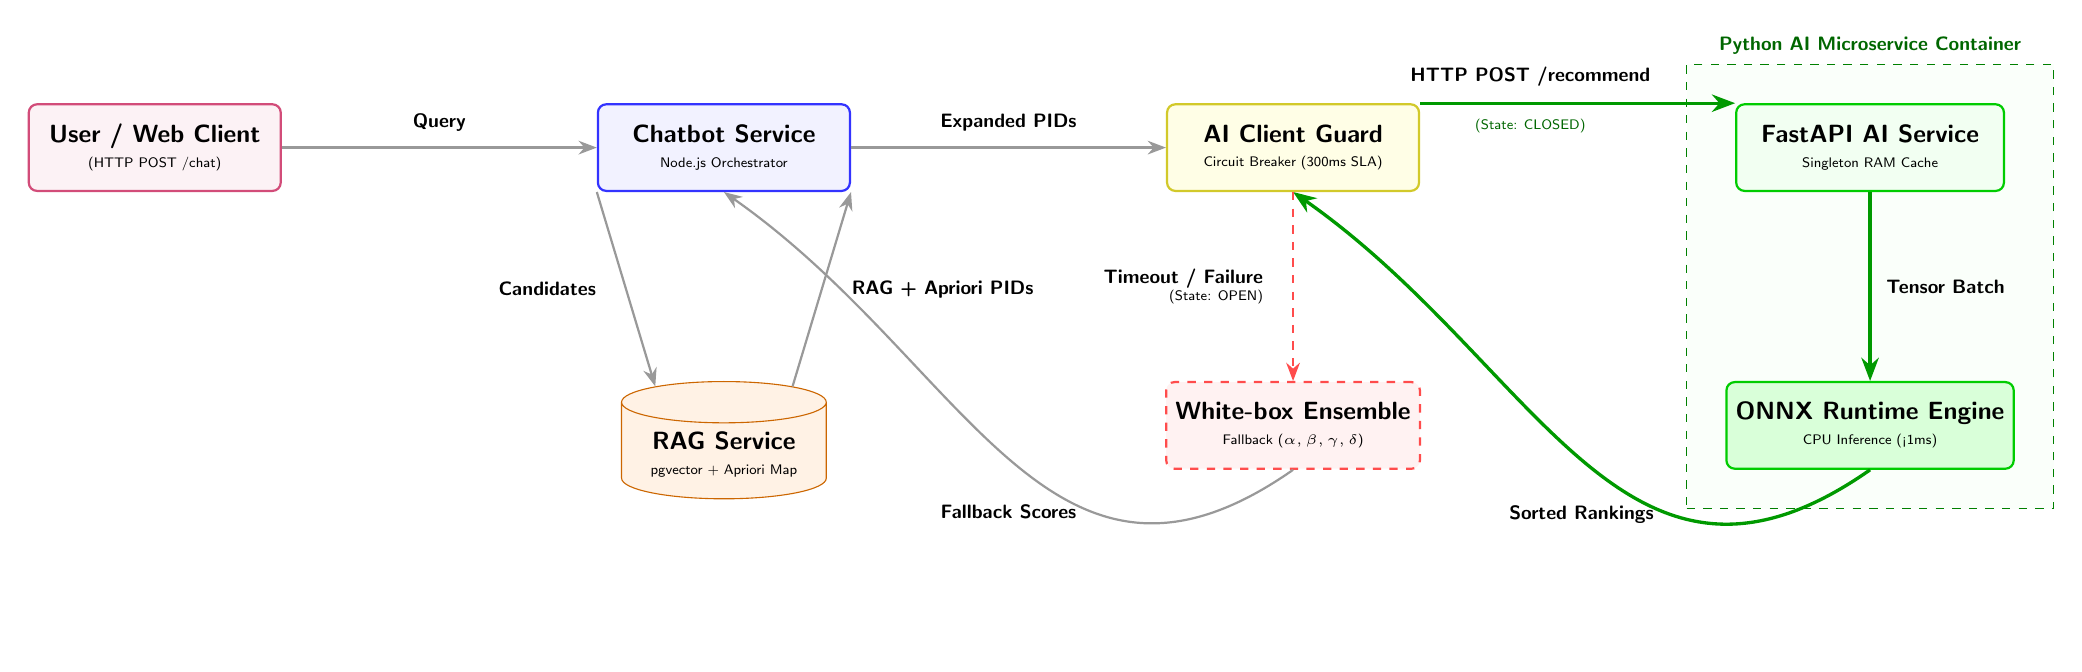
\begin{tikzpicture}[
    node distance=2.4cm and 4.0cm,
    font=\sffamily\small,
    box/.style={rectangle, draw=blue!80, fill=blue!5, thick, minimum width=3.2cm, minimum height=1.1cm, align=center, rounded corners=3pt},
    fastapi/.style={rectangle, draw=green!80!black, fill=green!5, thick, minimum width=3.4cm, minimum height=1.1cm, align=center, rounded corners=3pt},
    fallback/.style={rectangle, draw=red!70, fill=red!5, dashed, thick, minimum width=3.2cm, minimum height=1.1cm, align=center, rounded corners=3pt},
    storage/.style={cylinder, draw=orange!80!black, fill=orange!10, shape border rotate=90, aspect=0.25, minimum width=2.6cm, minimum height=1.1cm, align=center},
    arrow/.style={-Stealth, thick, draw=gray!80},
    fastarrow/.style={-Stealth, very thick, draw=green!60!black},
    failarrow/.style={-Stealth, thick, draw=red!70, dashed}
]

% --- NODES ---
\node (user) [box, fill=purple!5, draw=purple!70] {\textbf{User / Web Client}\\[-2pt]\tiny (HTTP POST /chat)};
\node (chatbot) [box, right=of user] {\textbf{Chatbot Service}\\[-2pt]\tiny Node.js Orchestrator};
\node (rag) [storage, below=2.4cm of chatbot] {\textbf{RAG Service}\\[-2pt]\tiny pgvector + Apriori Map};
\node (aiclient) [box, right=of chatbot, fill=yellow!10, draw=yellow!80!black] {\textbf{AI Client Guard}\\[-2pt]\tiny Circuit Breaker (300ms SLA)};
\node (fastapi) [fastapi, right=of aiclient] {\textbf{FastAPI AI Service}\\[-2pt]\tiny Singleton RAM Cache};
\node (onnx) [fastapi, fill=green!15, below=2.4cm of fastapi] {\textbf{ONNX Runtime Engine}\\[-2pt]\tiny CPU Inference (<1ms)};
\node (fallback) [fallback, below=2.4cm of aiclient] {\textbf{White-box Ensemble}\\[-2pt]\tiny Fallback ($\alpha, \beta, \gamma, \delta$)};

% --- CONNECTIONS ---

% 1. User -> Chatbot
\draw [arrow] (user) -- node[above=2pt, font=\scriptsize\bfseries]{Query} (chatbot);

% 2. Chatbot <-> RAG
\draw [arrow] (chatbot.south west) -- node[left=0.25cm, font=\scriptsize\bfseries]{Candidates} (rag.north west);
\draw [arrow] (rag.north east) -- node[right=0.25cm, font=\scriptsize\bfseries]{RAG + Apriori PIDs} (chatbot.south east);

% 3. Chatbot -> AI Client
\draw [arrow] (chatbot) -- node[above=2pt, font=\scriptsize\bfseries]{Expanded PIDs} (aiclient);

% 4. AI Client -> FastAPI (ĐÃ CHỈNH: pos=0.35 dịch nhãn về bên trái 35% chiều dài mũi tên)
\draw [fastarrow] (aiclient.north east) -- node[pos=0.35, above=2pt, font=\scriptsize\bfseries]{HTTP POST /recommend} 
                                         node[pos=0.35, below=2pt, font=\tiny, color=green!40!black]{(State: CLOSED)} (fastapi.north west);

% 5. FastAPI -> ONNX
\draw [fastarrow] (fastapi) -- node[right=2pt, font=\scriptsize\bfseries]{Tensor Batch} (onnx);

% 6. ONNX -> AI Client
\draw [fastarrow] (onnx.south) to[out=215, in=325, looseness=1.2] node[below=0.45cm, font=\scriptsize\bfseries, align=center]{Sorted Rankings} (aiclient.south);

% 7. Circuit Breaker Fallback
\draw [failarrow] (aiclient) -- node[left=0.25cm, font=\scriptsize, align=right]{\textbf{Timeout / Failure}\\[-2pt]\tiny (State: OPEN)} (fallback);

% 8. Fallback -> Chatbot
\draw [arrow] (fallback.south) to[out=215, in=325, looseness=1.2] node[below=0.45cm, font=\scriptsize\bfseries]{Fallback Scores} (chatbot.south);

% --- SUBGRAPH BACKGROUND ---
\begin{scope}[on background layer]
    \node [fit=(fastapi) (onnx), draw=green!50!black, fill=green!2, dashed, inner sep=14pt, label={[font=\scriptsize\bfseries, color=green!40!black]above:Python AI Microservice Container}] {};
\end{scope}

\end{tikzpicture}
\end{document}